\section{Trajectory Optimization}
Unfortunately due to the complex dynamics, large number of constraints and high dimensionality of the problem it is not possible to calculate the optimal orbital ascent trajectory analytically and thus numerical solutions are necessary. This has been a problem since the beginning of space exploration and thus countless years of research have resulted in the development of \emph{trajectory optimization}, a set of mathematical techniques used to find the ideal or desired behavior of a dynamical system by finding the inputs, referred to as \emph{controls}, to the system as functions of time.

The goal of trajectory optimization is to minimize an objective objective function in the form of $J(f(t))$, where $f(t)$ is an arbitrary vector function. In contrast, \emph{parameter optimization} minimizes objective functions in the form of $J(x)$, where $x$ is a vector of real numbers. This makes trajectory optimization a more difficult problem since the space of functions is much larger than a space of real numbers.

In itself trajectory optimization is class of methods used to compute solutions for optimal control problems. Within optimal control there are two types of solutions, closed-loop and open-loop. 


\begin{figure}[ht]			
	\centering
	

\tikzset{every picture/.style={line width=0.75pt}} %set default line width to 0.75pt        

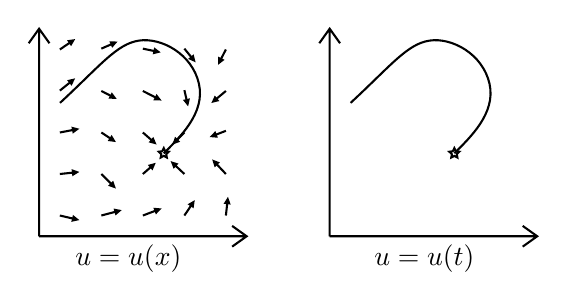
\begin{tikzpicture}[x=0.75pt,y=0.75pt,yscale=-1,xscale=1]
%uncomment if require: \path (0,300); %set diagram left start at 0, and has height of 300

%Shape: Axis 2D [id:dp39951459321449323] 
\draw  (10,105) -- (110,105)(10,5) -- (10,105) -- cycle (103,100) -- (110,105) -- (103,110) (5,12) -- (10,5) -- (15,12)  ;
%Straight Lines [id:da2517035703224979] 
\draw [line width=0.75]    (20,95) -- (26.48,96.52) ;
\draw [shift={(29.4,97.2)}, rotate = 193.17] [fill={rgb, 255:red, 0; green, 0; blue, 0 }  ][line width=0.08]  [draw opacity=0] (3.57,-1.72) -- (0,0) -- (3.57,1.72) -- cycle    ;
%Straight Lines [id:da9725014664238383] 
\draw [line width=0.75]    (20,75) -- (26.42,74.32) ;
\draw [shift={(29.4,74)}, rotate = 533.9300000000001] [fill={rgb, 255:red, 0; green, 0; blue, 0 }  ][line width=0.08]  [draw opacity=0] (3.57,-1.72) -- (0,0) -- (3.57,1.72) -- cycle    ;
%Straight Lines [id:da5860429978168766] 
\draw [line width=0.75]    (20,55) -- (26.45,53.76) ;
\draw [shift={(29.4,53.2)}, rotate = 529.1600000000001] [fill={rgb, 255:red, 0; green, 0; blue, 0 }  ][line width=0.08]  [draw opacity=0] (3.57,-1.72) -- (0,0) -- (3.57,1.72) -- cycle    ;
%Straight Lines [id:da11079150735885523] 
\draw [line width=0.75]    (20,34.82) -- (25.02,30.79) ;
\draw [shift={(27.36,28.91)}, rotate = 501.25] [fill={rgb, 255:red, 0; green, 0; blue, 0 }  ][line width=0.08]  [draw opacity=0] (3.57,-1.72) -- (0,0) -- (3.57,1.72) -- cycle    ;
%Straight Lines [id:da8837816203938313] 
\draw [line width=0.75]    (20,15) -- (24.91,11.68) ;
\draw [shift={(27.4,10)}, rotate = 505.95] [fill={rgb, 255:red, 0; green, 0; blue, 0 }  ][line width=0.08]  [draw opacity=0] (3.57,-1.72) -- (0,0) -- (3.57,1.72) -- cycle    ;
%Straight Lines [id:da5758737735521373] 
\draw [line width=0.75]    (40,95) -- (46.9,93.17) ;
\draw [shift={(49.8,92.4)}, rotate = 525.14] [fill={rgb, 255:red, 0; green, 0; blue, 0 }  ][line width=0.08]  [draw opacity=0] (3.57,-1.72) -- (0,0) -- (3.57,1.72) -- cycle    ;
%Straight Lines [id:da5516561087328649] 
\draw [line width=0.75]    (40,75) -- (44.88,79.88) ;
\draw [shift={(47,82)}, rotate = 225] [fill={rgb, 255:red, 0; green, 0; blue, 0 }  ][line width=0.08]  [draw opacity=0] (3.57,-1.72) -- (0,0) -- (3.57,1.72) -- cycle    ;
%Straight Lines [id:da7673401119897745] 
\draw [line width=0.75]    (40,55) -- (44.49,57.95) ;
\draw [shift={(47,59.6)}, rotate = 213.31] [fill={rgb, 255:red, 0; green, 0; blue, 0 }  ][line width=0.08]  [draw opacity=0] (3.57,-1.72) -- (0,0) -- (3.57,1.72) -- cycle    ;
%Straight Lines [id:da7321931625560845] 
\draw [line width=0.75]    (40,35) -- (44.73,37.43) ;
\draw [shift={(47.4,38.8)}, rotate = 207.18] [fill={rgb, 255:red, 0; green, 0; blue, 0 }  ][line width=0.08]  [draw opacity=0] (3.57,-1.72) -- (0,0) -- (3.57,1.72) -- cycle    ;
%Straight Lines [id:da8653846903313711] 
\draw [line width=0.75]    (40,14.6) -- (45.05,12.4) ;
\draw [shift={(47.8,11.2)}, rotate = 516.45] [fill={rgb, 255:red, 0; green, 0; blue, 0 }  ][line width=0.08]  [draw opacity=0] (3.57,-1.72) -- (0,0) -- (3.57,1.72) -- cycle    ;
%Straight Lines [id:da40204656641388303] 
\draw [line width=0.75]    (60,95) -- (66.19,92.66) ;
\draw [shift={(69,91.6)}, rotate = 519.3] [fill={rgb, 255:red, 0; green, 0; blue, 0 }  ][line width=0.08]  [draw opacity=0] (3.57,-1.72) -- (0,0) -- (3.57,1.72) -- cycle    ;
%Straight Lines [id:da7612220292173184] 
\draw [line width=0.75]    (60,75) -- (63.94,71.57) ;
\draw [shift={(66.2,69.6)}, rotate = 498.95] [fill={rgb, 255:red, 0; green, 0; blue, 0 }  ][line width=0.08]  [draw opacity=0] (3.57,-1.72) -- (0,0) -- (3.57,1.72) -- cycle    ;
%Straight Lines [id:da19814629412224938] 
\draw [line width=0.75]    (60,55) -- (64.35,58.82) ;
\draw [shift={(66.6,60.8)}, rotate = 221.31] [fill={rgb, 255:red, 0; green, 0; blue, 0 }  ][line width=0.08]  [draw opacity=0] (3.57,-1.72) -- (0,0) -- (3.57,1.72) -- cycle    ;
%Straight Lines [id:da0727741582230601] 
\draw [line width=0.75]    (60,35) -- (66.33,38.23) ;
\draw [shift={(69,39.6)}, rotate = 207.07] [fill={rgb, 255:red, 0; green, 0; blue, 0 }  ][line width=0.08]  [draw opacity=0] (3.57,-1.72) -- (0,0) -- (3.57,1.72) -- cycle    ;
%Straight Lines [id:da5304237193507622] 
\draw [line width=0.75]    (60,14.6) -- (65.66,15.79) ;
\draw [shift={(68.6,16.4)}, rotate = 191.82] [fill={rgb, 255:red, 0; green, 0; blue, 0 }  ][line width=0.08]  [draw opacity=0] (3.57,-1.72) -- (0,0) -- (3.57,1.72) -- cycle    ;
%Straight Lines [id:da09925906152117014] 
\draw [line width=0.75]    (80,95) -- (83.32,90.09) ;
\draw [shift={(85,87.6)}, rotate = 484.05] [fill={rgb, 255:red, 0; green, 0; blue, 0 }  ][line width=0.08]  [draw opacity=0] (3.57,-1.72) -- (0,0) -- (3.57,1.72) -- cycle    ;
%Straight Lines [id:da17642668844242926] 
\draw [line width=0.75]    (80,75) -- (75.59,70.85) ;
\draw [shift={(73.4,68.8)}, rotate = 403.21000000000004] [fill={rgb, 255:red, 0; green, 0; blue, 0 }  ][line width=0.08]  [draw opacity=0] (3.57,-1.72) -- (0,0) -- (3.57,1.72) -- cycle    ;
%Straight Lines [id:da9829859509621575] 
\draw [line width=0.75]    (80,55) -- (76.32,58.68) ;
\draw [shift={(74.2,60.8)}, rotate = 315] [fill={rgb, 255:red, 0; green, 0; blue, 0 }  ][line width=0.08]  [draw opacity=0] (3.57,-1.72) -- (0,0) -- (3.57,1.72) -- cycle    ;
%Straight Lines [id:da03714071169973421] 
\draw [line width=0.75]    (80,34.6) -- (81.13,39.48) ;
\draw [shift={(81.8,42.4)}, rotate = 257.01] [fill={rgb, 255:red, 0; green, 0; blue, 0 }  ][line width=0.08]  [draw opacity=0] (3.57,-1.72) -- (0,0) -- (3.57,1.72) -- cycle    ;
%Straight Lines [id:da5095897243936336] 
\draw [line width=0.75]    (80,14.6) -- (83.5,18.88) ;
\draw [shift={(85.4,21.2)}, rotate = 230.71] [fill={rgb, 255:red, 0; green, 0; blue, 0 }  ][line width=0.08]  [draw opacity=0] (3.57,-1.72) -- (0,0) -- (3.57,1.72) -- cycle    ;
%Straight Lines [id:da09008695828668767] 
\draw [line width=0.75]    (100,95) -- (100.67,88.98) ;
\draw [shift={(101,86)}, rotate = 456.34] [fill={rgb, 255:red, 0; green, 0; blue, 0 }  ][line width=0.08]  [draw opacity=0] (3.57,-1.72) -- (0,0) -- (3.57,1.72) -- cycle    ;
%Straight Lines [id:da16314992167885833] 
\draw [line width=0.75]    (100,75) -- (95.46,70.18) ;
\draw [shift={(93.4,68)}, rotate = 406.68] [fill={rgb, 255:red, 0; green, 0; blue, 0 }  ][line width=0.08]  [draw opacity=0] (3.57,-1.72) -- (0,0) -- (3.57,1.72) -- cycle    ;
%Straight Lines [id:da8997659499815567] 
\draw [line width=0.75]    (100,54.2) -- (95,56.12) ;
\draw [shift={(92.2,57.2)}, rotate = 338.96000000000004] [fill={rgb, 255:red, 0; green, 0; blue, 0 }  ][line width=0.08]  [draw opacity=0] (3.57,-1.72) -- (0,0) -- (3.57,1.72) -- cycle    ;
%Straight Lines [id:da7968704721077784] 
\draw [line width=0.75]    (100,35) -- (95.31,38.89) ;
\draw [shift={(93,40.8)}, rotate = 320.36] [fill={rgb, 255:red, 0; green, 0; blue, 0 }  ][line width=0.08]  [draw opacity=0] (3.57,-1.72) -- (0,0) -- (3.57,1.72) -- cycle    ;
%Straight Lines [id:da30383591371467555] 
\draw [line width=0.75]    (100,15) -- (97.57,19.73) ;
\draw [shift={(96.2,22.4)}, rotate = 297.18] [fill={rgb, 255:red, 0; green, 0; blue, 0 }  ][line width=0.08]  [draw opacity=0] (3.57,-1.72) -- (0,0) -- (3.57,1.72) -- cycle    ;
%Shape: Star [id:dp04672232148485023] 
\draw   (70.07,62.53) -- (70.8,64.02) -- (72.45,64.26) -- (71.26,65.42) -- (71.54,67.05) -- (70.07,66.28) -- (68.6,67.05) -- (68.88,65.42) -- (67.69,64.26) -- (69.33,64.02) -- cycle ;
%Curve Lines [id:da18491075498888065] 
\draw    (20.09,40.73) .. controls (39.55,22.73) and (47.36,12.36) .. (58.09,10.73) .. controls (68.82,9.09) and (83.73,17.09) .. (87,31.45) .. controls (90.27,45.82) and (77.36,57.64) .. (70.07,65.03) ;
%Shape: Axis 2D [id:dp42032936326001513] 
\draw  (150,105) -- (250,105)(150,5) -- (150,105) -- cycle (243,100) -- (250,105) -- (243,110) (145,12) -- (150,5) -- (155,12)  ;
%Shape: Star [id:dp26772001548097313] 
\draw   (210.07,62.53) -- (210.8,64.02) -- (212.45,64.26) -- (211.26,65.42) -- (211.54,67.05) -- (210.07,66.28) -- (208.6,67.05) -- (208.88,65.42) -- (207.69,64.26) -- (209.33,64.02) -- cycle ;
%Curve Lines [id:da5681106290117939] 
\draw    (160.09,40.73) .. controls (179.55,22.73) and (187.36,12.36) .. (198.09,10.73) .. controls (208.82,9.09) and (223.73,17.09) .. (227,31.45) .. controls (230.27,45.82) and (217.36,57.64) .. (210.07,65.03) ;

% Text Node
\draw (26,107.4) node [anchor=north west][inner sep=0.75pt]    {$u=u( x)$};
% Text Node
\draw (170,107.4) node [anchor=north west][inner sep=0.75pt]    {$u=u( t)$};


\end{tikzpicture}
			
	\caption{Optimal control closed and open loop solutions.}
	\label{fig:pow_fly_trj_an}
\end{figure}

Closed-loop solutions provide the optimal controls for the entire state space, $u(x)$, thus advantages of these solutions include the possibility to compute the global optimal solution and the ability to apply the solution directly into real systems. The drawback is that these methods are difficult to compute specially when applied to higher dimensional problems. \acrlong{dp} and the main topic of thesis, \acrlong{rl} work by finding an optimal policy. This is a deterministic function or probability distribution mapping states to actions and thus provide closed-loop solutions to optimal control problems. Chapter~\ref{ch:rl} continues further with these methods.

On the other hand open loop solutions consist of an initial state and a sequence of controls defined as a function of time, $u(t)$. Together these define a single trajectory the system takes through the state space. The advantage of these solutions is that they are easier to compute, and thus more practical for higher dimensional problems. The disadvantage is that these solutions do not necessarily converge to the global optimal



